\section*{System Features and Capabilities}

\textbf{THERAPY} is designed to be modular, extensible, and user-centric. Each component contributes to the therapeutic feedback loop — enhancing emotional clarity, therapeutic continuity, and ethically grounded data integration.

\bigskip

\noindent\textbf{Client-Facing Features}

\begin{itemize}
  \item \textbf{Mood Check-ins} — Quick 1–10 scale entries with optional context, submitted daily or on demand.
  \item \textbf{Guided Journaling} — Prompts tailored to emotional state, trauma sensitivity, and personal goals.
  \item \textbf{Progress Visualizations} — Trend charts and summaries that reflect emotional fluctuations over time.
  \item \textbf{Personal Insights Feed} — Private, AI-generated reflections and reframings based on journal content.
  \item \textbf{Education Portal} — Curated psychoeducation on CBT, emotional literacy, somatic grounding, and more.
\end{itemize}

\bigskip

The THERAPY mobile app serves as the client’s daily companion — a private, intuitive space for emotional tracking, guided self-reflection, and ongoing learning. Its design prioritizes simplicity, safety, and autonomy, empowering individuals to externalize emotions without judgment or oversharing. The app’s core interface adapts dynamically to mood trends and journal themes, offering timely prompts and visual feedback in support of each user’s therapeutic goals.

\begin{figure}[H]
  \centering
  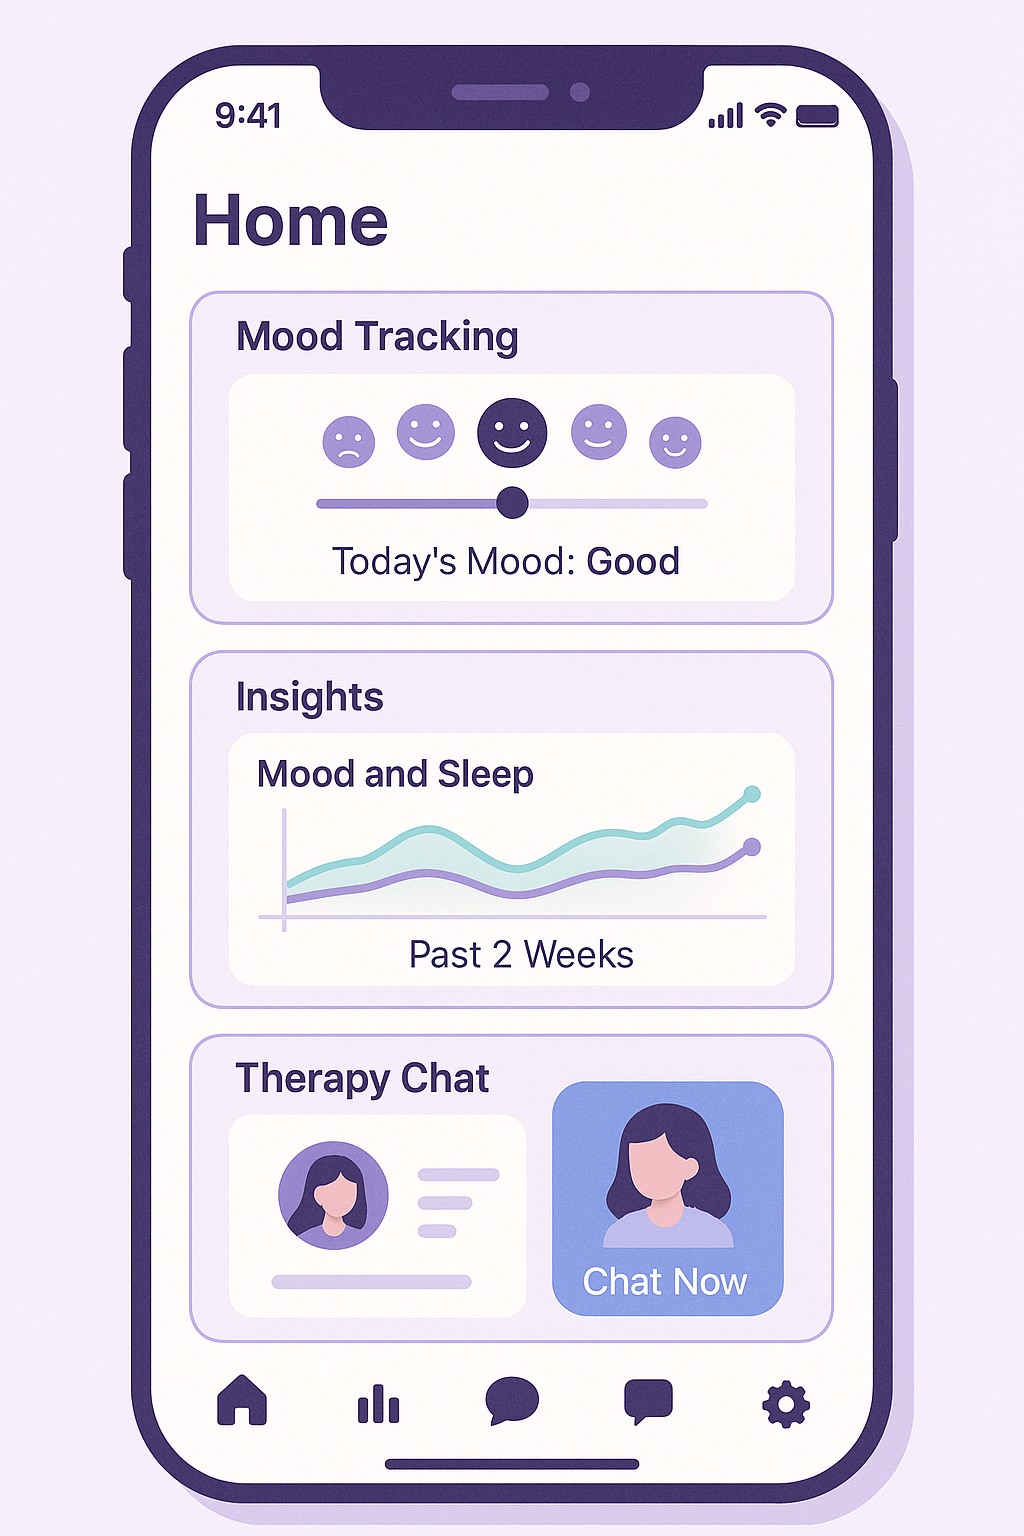
\includegraphics[width=0.65\textwidth]{features_client_mockup.png}
  \caption{Mobile interface showcasing journaling, mood tracking, and visual feedback}
\end{figure}

\bigskip

\noindent\textbf{Therapist Dashboard Features}

\begin{itemize}
  \item \textbf{Client Summary View} — Weekly emotional overviews including mood trajectories, topic themes, and AI-inferred flags.
  \item \textbf{Session Preparation Feed} — Highlights key journal moments, shifts in tone, and detected distortions.
  \item \textbf{Historical Context} — A continuity timeline to revisit long-term patterns and themes.
  \item \textbf{Secure Messaging} — Short-form, scoped communication between sessions with rate limiting.
  \item \textbf{Insight Acknowledgement} — A private space for therapists to log notes before or after sessions.
\end{itemize}

\begin{figure}[H]
  \centering
  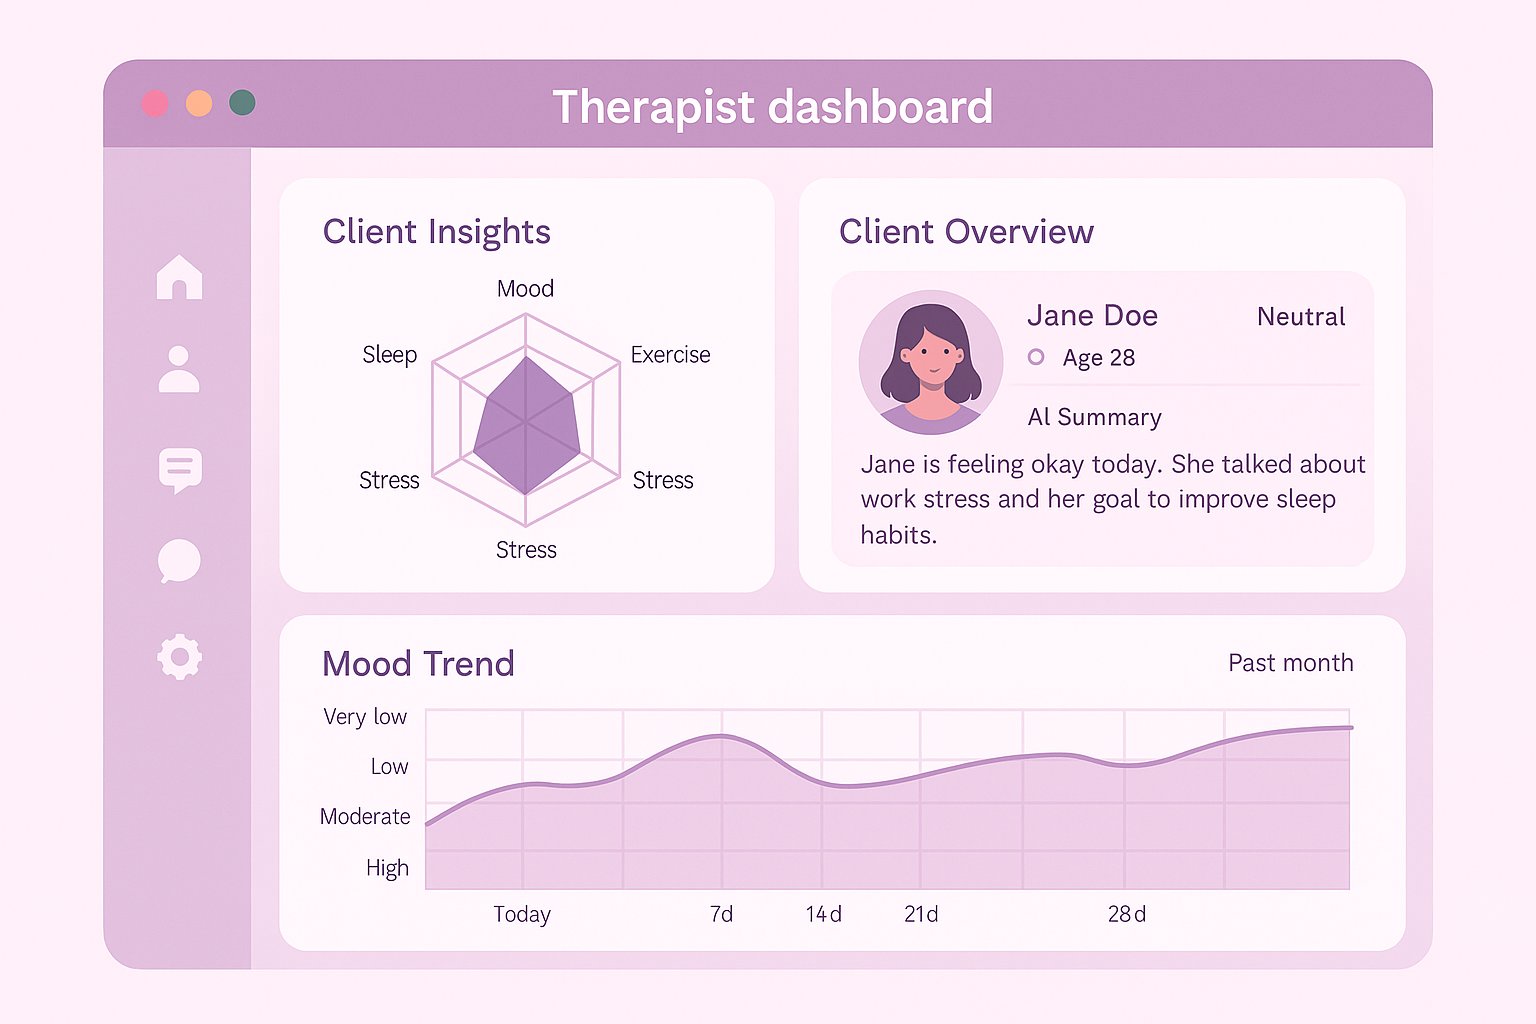
\includegraphics[width=0.85\textwidth]{features_therapist_dashboard.png}
  \caption{Therapist dashboard showing emotional trends, AI flags, and session insights}
\end{figure}

\bigskip

\noindent\textbf{System-Level Infrastructure}

\begin{itemize}
  \item \textbf{AI Summarization Engine} — Leverages fine-tuned large language models aligned with therapeutic tone and language.
  \item \textbf{Privacy-First Data Model} — End-to-end encryption, opt-in logging, and user-controlled sharing preferences.
  \item \textbf{Modular API Layer} — Supports integrations with EHRs, research platforms, or digital therapeutics.
  \item \textbf{Open-Source Core} — Transparent, extensible, and available for nonprofit, academic, and clinical deployment.
\end{itemize}

\begin{figure}[H]
  \centering
  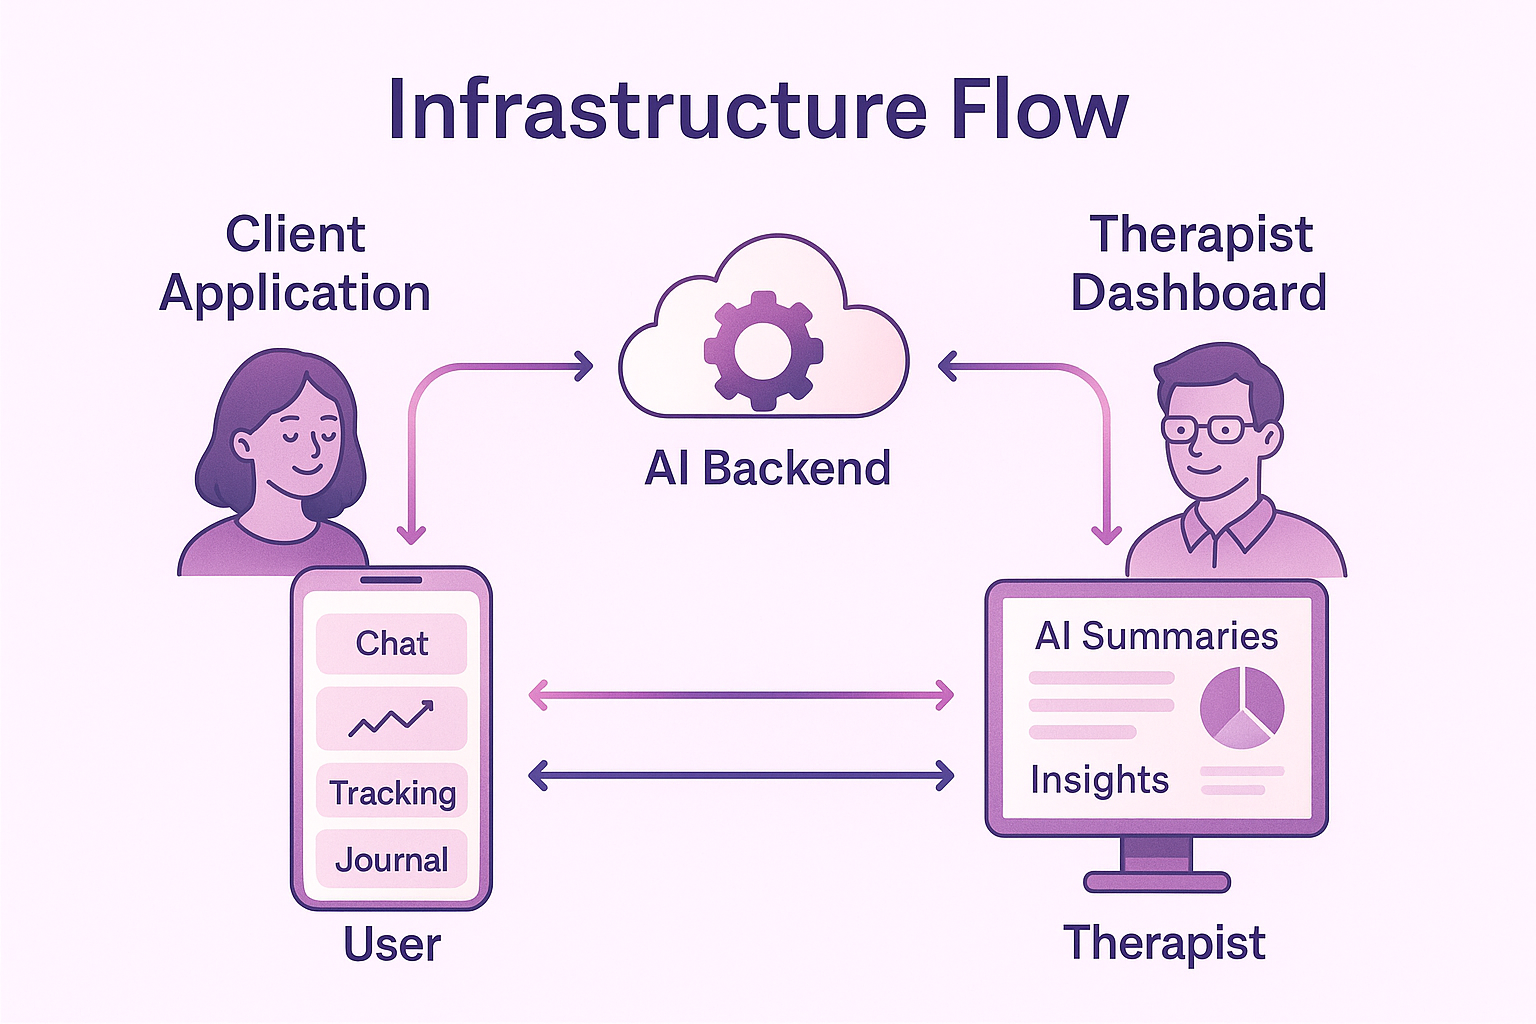
\includegraphics[width=0.85\textwidth]{features_infrastructure_flow.png}
  \caption{High-level system diagram showing THERAPY's backend architecture and data flow}
\end{figure}
